\section{Erzeugung der Trace-Datei}
\label{section:Erzeugung der Trace-Datei}
\begin{itemize}
    \item Definition der notwendigen Informationen der Trace-Datei
    \item Aufzeigen der Herausforderungen in Bezug auf Performance und
    Speicherauslastung
  \item Anforderungen definieren:
  \begin{itemize}
    \item Laufzeit des Programms soll sich um maximal x\% erhöhen
    \item Speicherauslastung des Programms soll sich um maximal y\% erhöhen
  \end{itemize}
    \item Aktuelle Idee: Das Erstellen der Trace-Datei wird in der
    Laufzeitumgebung umgesetzt. Die Implementierung erfolgt in einer eigenen
    Klasse und kann aktiviert oder deaktiviert sein. Die Klasse wird von der
    Semaphore Implementierung der Laufzeitumgebung verwendet werden. Beim Aufruf
    von Request oder Release wird geprüft, ob die Informationen geloggt werden
    sollen. Falls das Logging aktiviert ist, werden die Informationen in eine
    Warteschlange eingereiht. Die Warteschlange wird eine Datenstruktur
    verwendet, welche das Hinzufügen, Entfernen und das Abfragen der aktuellen
    Größe mit der Komplexität O(1) implementiert. Bei jeder x-ten Aktivierung,
    wobei x die maximale Größe der Warteschlange ist, werden alle vorhanden
    Einträge aus der Warteschlange entfernt und in die Trace-Datei geschrieben.
    Die Liste wird für jeden Eintrag einmal durchlaufen. Die Laufzeit beträgt
    daher O(x). Das Öffnen und Schließen der Trace-Datei hat die Laufzeit y. Das
    Schreiben eines Logeintrags, also eine Zeile in die Trace-Datei, hat die
    Laufzeit z. Damit hat jeder x-te Request/Release Aufruf die Laufzeit O(y + x
    $\cdot$ z). Somit hat jeder Request/Release Aufruf die Laufzeit O($\frac{y +
    x \cdot z}{x}$).

    Zusätzlich zu jedem x-ten Request/Release Aufruf das Schreiben in die
    Trace-Datei auch zeitich angestoßen werden. Zum Beispiel sollte alle 60
    Sekunden oder nach x Aufrufen die Warteschlange geleert und in die
    Trace-Datei geschrieben werden. Bei jedem x-ten Request/Release Aufruf muss
    der Timer der Warteschlange wieder zurückgesetzt werden. Bedeutet wenn nach
    50 Sekunden der x-te Aufruf kommt, muss der Timer wieder von vorne beginnen,
    damit die Trace-Datei nicht nach 10 Sekunden erneut beschrieben wird.

    Der zusätzliche Speicherbedarf beträgt $x \cdot i$, wobei i die Größe der
    Information eines Logeintrags entspricht. Ein Logeintrag benötigt die
    Informationen:
    \begin{enumerate}
      \item Aktion (Thread Start, Request, Release) => 32 Bit (enum)
      \item ID des Threads => 16-Bit Ganzzahl (maximale Thread Id für Linux
      beträgt 32768) theoretisch über 15 Bit abbildbar, da immer positiv
      \item Name des Lockobjekts => 16-Bit Ganzzahl (theoretisch über 11 Bit
      Ganzzahl abbildbar) (maximal Variablennamenlänge für C++ beträgt 2048)
    \end{enumerate}
    Mindestgröße für i beträgt 32 + 16 + 16 = 64 Bit. Die Warteschlange benötigt
    maximal daher 64 Bit $\cdot$ x zusätzlichen Speicher.
\end{itemize}

\begin{figure}[ht]
  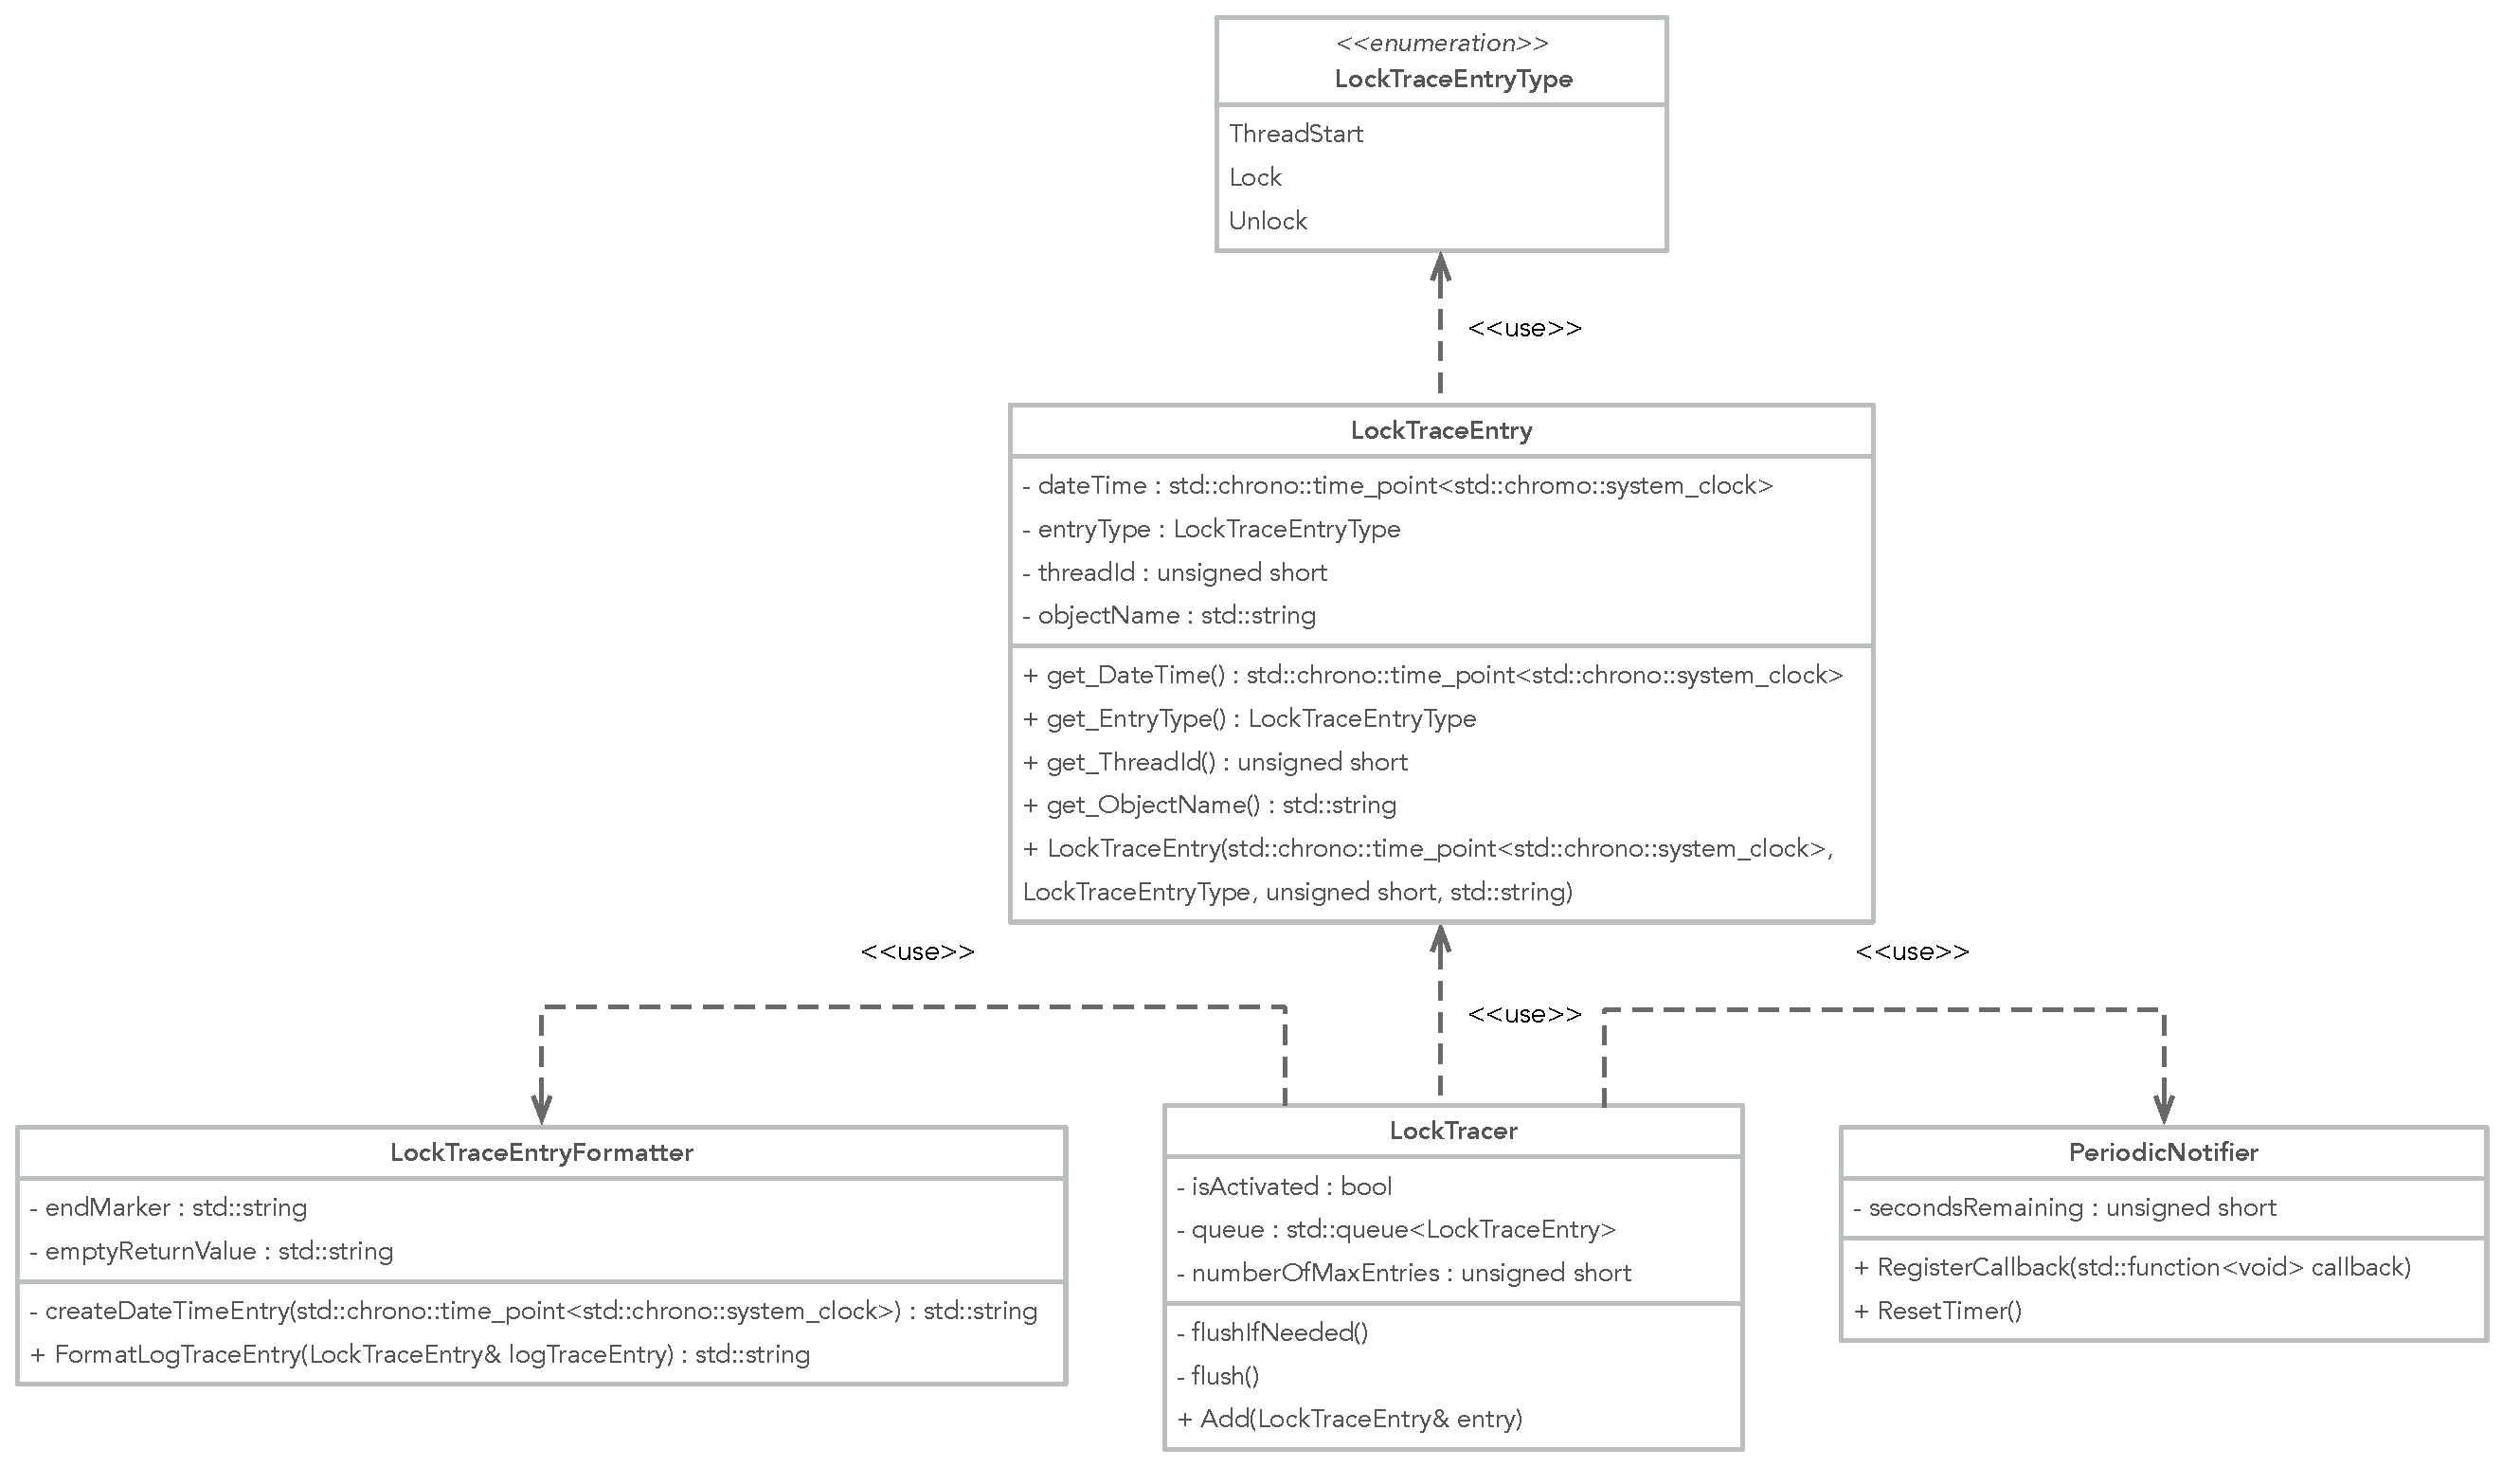
\includegraphics[width=\linewidth]{LockTrace_Design.eps}
  \caption{UML Klassendiagramm für die Erzeugung der Trace-Datei}
  \label{fig:LockTrace_Design}
\end{figure}

\section{Analysieren der Trace-Datei}
\label{section:Analysieren der Trace-Datei}
\begin{itemize}
  \item Externes Programm geschrieben in Java
  \item Anforderungen definieren:
  \begin{itemize}
    \item Darstellung der Trace-Datei (welcher Thread hat welches
    Synchronisationsmittel wann genommen und wieder freigegeben) 
  \end{itemize}
\end{itemize}

\section{Erweiterung: Potenzielle Deadlocks}
\label{section:Erweiterung: Potenzielle Deadlocks}
\begin{itemize}
  \item Programm aus \cref{section:Analysieren der Trace-Datei} wird erweitert
  \item Es sollen potenzielle Deadlocks mit Hilfe des aus \cref{section:MagicLock}
 beschriebenen Verfahrens bestimmt werden
  \item Potenzielle Deadlocks sollen als gerichtete Graphen visualisiert werden
\end{itemize}